% !TeX spellcheck = en_GB

\section{Requirements}\label{sec:requirements}

The following sections describe the primary requirements in the form of quality user stories.
Figure \ref{fig:requirements-overview} shows an overview of the primary use cases.

\begin{figure}[h]
    \centering
    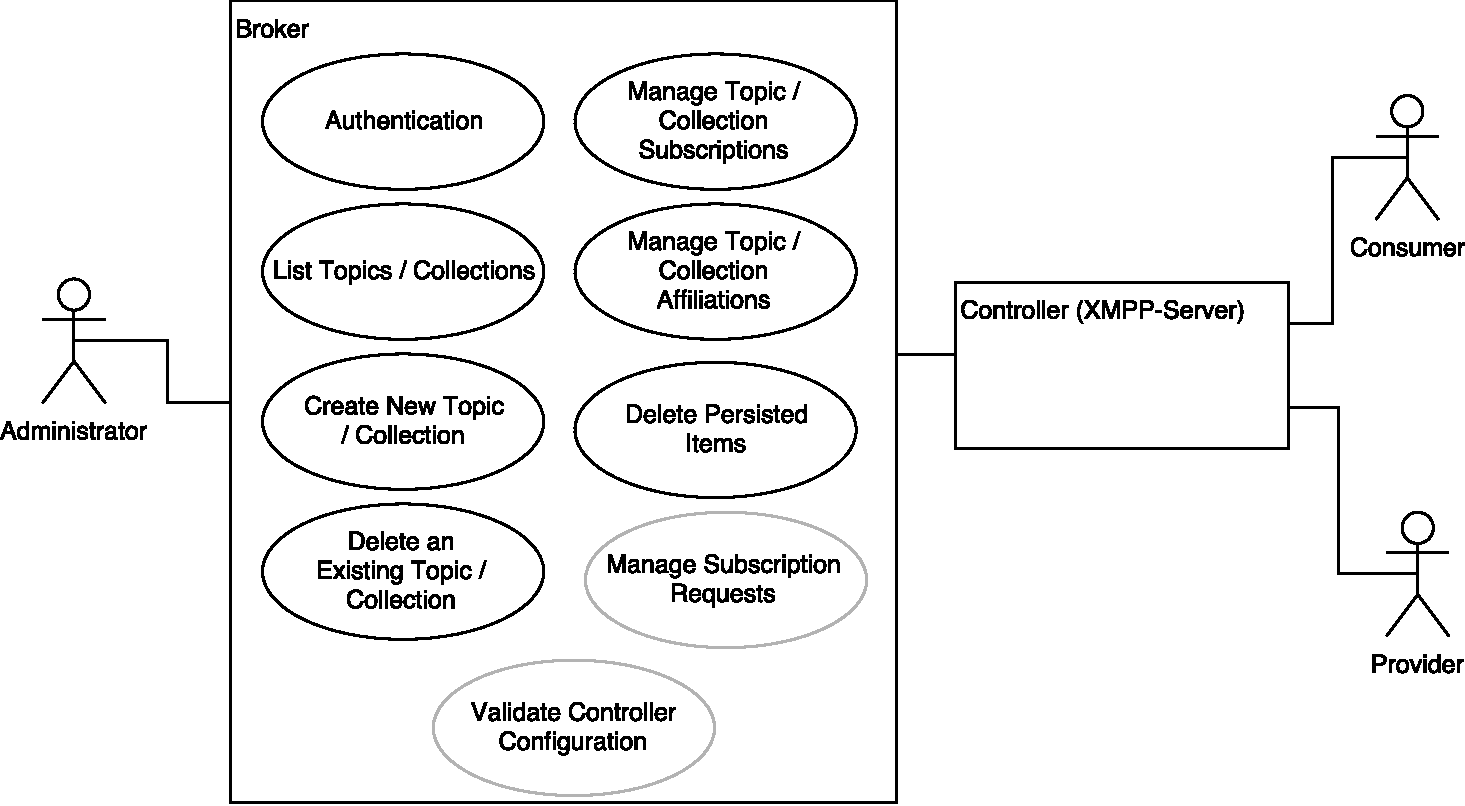
\includegraphics[width=1\linewidth]{resources/requirements_overview}
    \caption{UML Use Case Diagram presenting an overview of the primary component.}
    \label{fig:requirements-overview}
\end{figure}


\subsection{01: Login}

As an Administrator,\\
I would like to log in\\
so that only I can inspect and manage topics.\\
To achieve this goal, I expect the following qualities (in descending order of priority):

\begin{itemize}
    \item The authentication time must on average not take 50\% longer than a regular XMPP-login from the client.
\end{itemize}

\noindent To be clarified:

\begin{itemize}
    \item It would be convenient to not maintain a separate user database and to use the same credentials for authentication
            as for the XMPP server and just forward them. This is from a security perspective usually not a great idea. Are there any
            specific requirements?
\end{itemize}

\subsection{01a: Secure XMPP Connection}

As an administrator concerned with security requirements,\\
I would like to use either SASL EXTERNAL or SASL SCRAM mechanism for authentication - \\
\begin{itemize}
    \item preferably the SCRAM-SHA-256-PLUS variant and
    \item preferably using mutual certificate-based authentication including revocation status checking
\end{itemize}

\noindent - so that the controller benefits from:

\begin{itemize}
    \item full accordance with the XMPP grid draft~\cite{ietf-mile-xmpp-grid-05}
    \item maximal security standards
\end{itemize}

\noindent To achieve this goal, I am willing to accept:
\begin{itemize}
    \item More costly and less user friendly authentication
    \item limited compatibility of supported XMPP servers
\end{itemize}

\subsection{02: Logout}

As an Administrator,\\
I would like to log out\\
to terminate a session.

\subsection{03: List available topics}

\subsection{04: Create a new topic}

\subsection{05: Delete an existing topic}

\subsection{06: Manage topic subscriptions}

\subsection{07: Manage topic affiliations}

\subsection{08: Manage pending subscription requests}

\subsection{09: Delete persisted Item in a Topic}

\subsection{10: Purge persisted Items in a Topic}

\subsection{11: Validate controller configuration}





% (Disco checks)

% \subsection{01: Login}

% As a [role],\\
% I would like to [goal]\\
% so that [effect (business value, impact)].\\
% To achieve this goal, I expect the following qualities (in descending order of priority):

% \begin{itemize}
%     \item measurable usability quality property, e.g. input steps required to complete story
%     \item measurable performance quality, e.g. average and worst case story response time
%     \item other verifiable quality goal if measurements are considered too risky/costly
% \end{itemize}


